\speaker{\Mathieu}

\begin{frame}
\frametitle{M\underline{V}C : Les vues}
\begin{figure}[!h]
	\begin{center}
	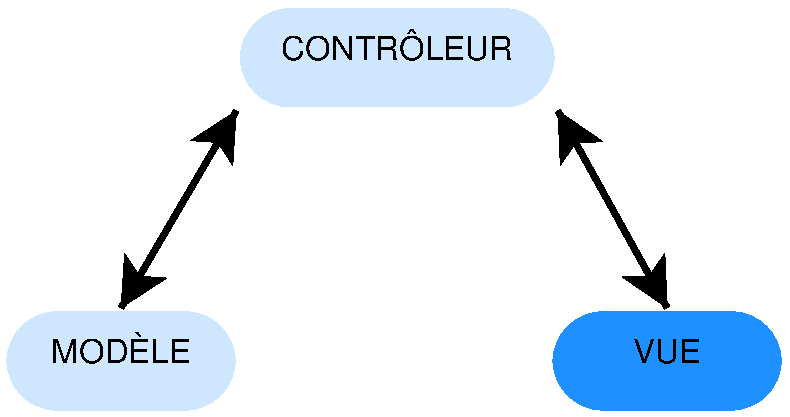
\includegraphics[scale=0.5]{images/mvcVue}
	\caption{Architecture M\underline{V}C}
	\end{center}
\end{figure}
Vue : partie visible, IHM(Interface Homme Machine)
\end{frame}

\begin{frame}
\frametitle{M\underline{V}C : Les vues}
\begin{block}{Vocabulaire}
\textbf{Template} : définit l'habillage d'une page, la position de ses éléments
\end{block}
\begin{figure}[!h]
	\begin{center}
	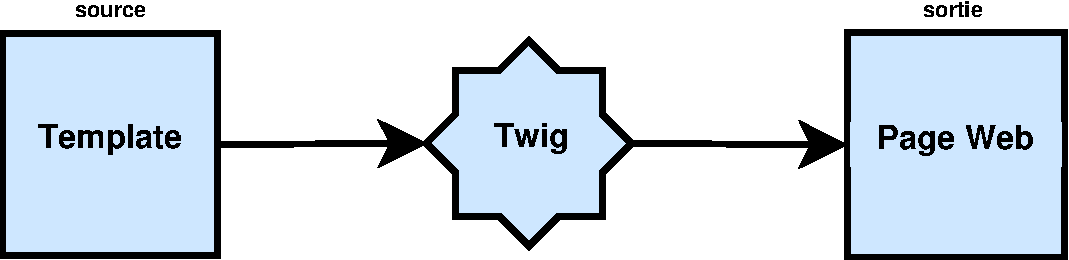
\includegraphics[scale=0.5]{images/twig}
	\caption{Fonctionnement du moteur de template Twig}
	\end{center}
\end{figure}
\end{frame}

\begin{frame}
\frametitle{M\underline{V}C : Les vues}
\begin{block}{Organisation des templates}

\end{block}
\end{frame}